\documentclass{knittingpattern}
\usepackage[utf8]{inputenc}
\usepackage{graphicx}
\usepackage{xskak}
\usepackage{chemfig}
\usepackage{modiagram}
\usepackage[siunitx]{circuitikz}
\usepackage{amssymb}
\usepackage{amsmath}
\usepackage{fancyhdr}
\usepackage{tikz}
\usepackage[dvipsnames]{xcolor}
\usetikzlibrary{automata, positioning,arrows}
\usepackage{tikz}
\usepackage[dvipsnames]{xcolor}

\definecolor{colour0}{HTML}{000000}
\definecolor{colour1}{HTML}{FBC02D}
\definecolor{colour2}{HTML}{C39BD3}
\definecolor{colour3}{HTML}{82E0AA}
\definecolor{colour4}{HTML}{D2B4DE}
\title{IT Workshop Assignment }

\author{SUSMITHA BAIRA\\B191984\\CSE 021-C1}


\date{August 2022}





\begin{document}
\maketitle\vskip-15pt\hrule\vskip15pt
\section{ Knitting Patterns}
This class provides a very convenient way to introduce boxed diagrams. We are thus going to use our stock image a few more
times. Also,it has a few features to make knitting instructions more readable, however, we can adapt them to make prettier
documents for our purposes as well.
\begin{figure}[h]
    \centering
    \setlength{\fboxsep}{15pt}
    \setlength{\fboxrule}{2pt}
\fbox{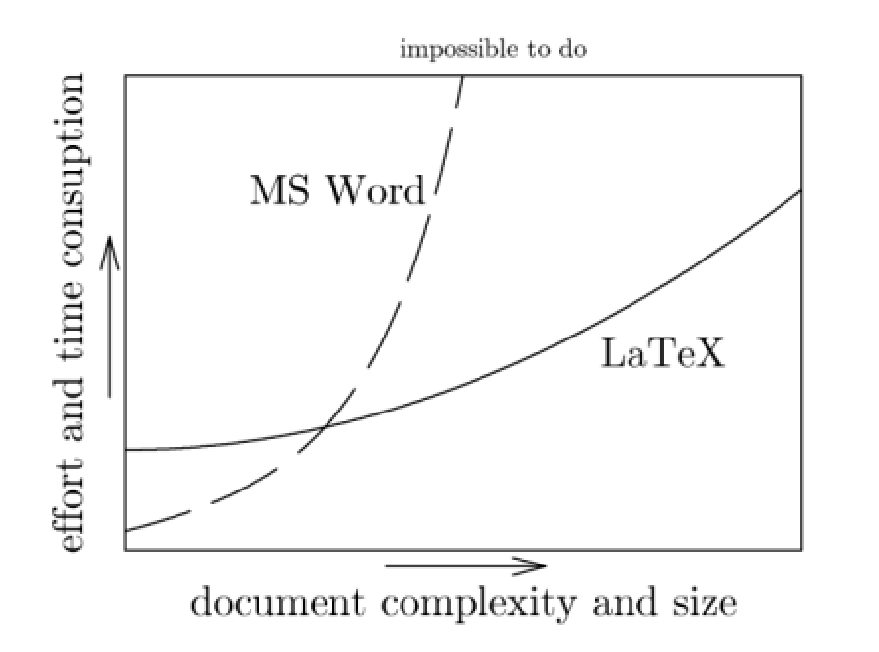
\includegraphics[scale=0.35]{pic2.png}}
\end{figure}
\important{colour0}{colour1}{We have a way of highlighting important text, or as was originally intended, important
instructions. Feel free to choose whatever background and border colour you like when
you replicate these features, but try to replicate the dimensions as well as you can.}
\begin{pattern}{colour2}{colour3}
\textbf{Course}&\textbf{Credits}\\
Introduction to Computer Programming&6\\
Abstraction and Paradigms in Programming&6\\
Abstractions and Paradigms in Programming Lab&3\\
Data Structure and Algorithms&6\\
Software Systems Lab &8\\
\end{pattern}
\important{colour0}{colour4}{\underline{Note}

This is a note. The above feature was introduced to typeset a sequence of knitting instructions.
The first column is for the instruction, the second for the number of stitches. But hey, it looks
cool}
\begin{minipage}{0.1\textwidth}
\begin{figure}[H]
\setlength{\fboxsep}{17pt}
\setlength{\fboxrule}{1.5pt}
\fbox{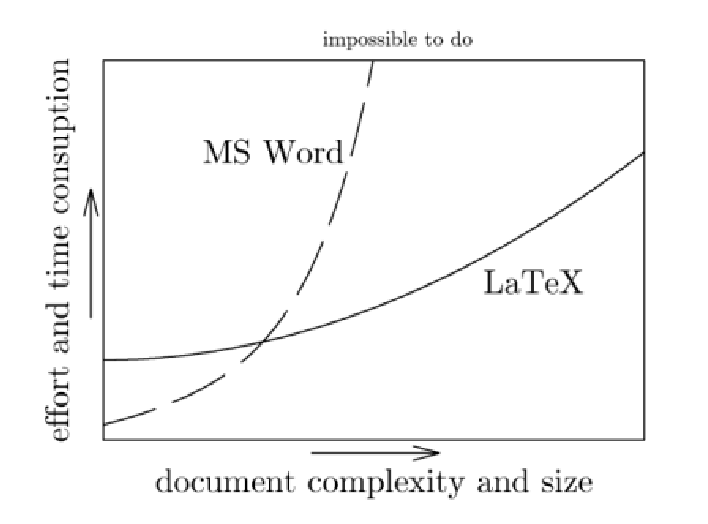
\includegraphics[width=7.5cm,height=5cm]{picb.png}}
\end{figure}
\end{minipage} \hfill
\begin{minipage}{0.5\textwidth}
Look at the adjoining graph. Yes, you’ve seen it before. This \\ time, it is side by side with a paragraph! And there’s a beautiful box around it! By default, this will be a quarter of the
width of the page. If you follow the hint that is the title of this section, you won’t have to type in cumbersome code to fit in images. Also, have you noticed that the pages are much
wider? A lot of it will be clear when you read up on the knittingpatterns class. It is already available with the MacTeX distributions, and of course, online on Overleaf. If your distribution does not offer it, download it from here and copy the .cls file to the folder/directory your code is in. See the point where stuff becomes exponentially harder to do without LATEX? We daresay the rest of this assignment crosses that point. Good luck!

\end{minipage}
\newpage
\section{\textbf{Chess Notation}}
\begin{center}
\textbf{Adolf Anderssen - Lionel Kieseritzky}\\
London, 1851\\
\newchessgame
\setchessboard{boardfontsize=18}
\chessboard[setfen=rnb1k1nr/p2p1ppp/3B/1pbN1N1P/4P1P/3P1Q/PqP/R4kR]\\
\end{center}
In this position, Black played  \textbf{18. . .\symbishop }xg1, taking the rook. Had he opted for 18. . . \symqueen xa1, he would be better, but still in
trouble. However, his choice allowed for a spectacular finish. \textbf{19 e5!} Blunting the Queen’s protection of g7. \textbf{19. . . \symqueen xa1+}.
What else? The rook is en-prise.\textbf{ 20 \symking e2 \symknight a6.} This covers the c7 square, as White was threatening Mate in 2, example like 20. . . h6\textbf{ 21 \symknight xg7+ \symking d8 22 \symbishop c7\#. 21 \symknight xg7+ \symking d8 22 \symqueen f6+!}
\begin{center}
\newchessgame
\setchessboard{boardfontsize=18}
\chessboard[setfen=r1bk2nr/p2p1pNp/n2B1Q/1p1NP2P/6P/3P/P1P1K/q5b]
\end{center}
A brilliant Queen sacrifice to deflect the Knight on g8 that protects \textbf{e7 22. . . \symknight xf6 23 \symbishop e7}\#
\begin{center}
    \newchessgame
    \setchessboard{boardfontsize=18}
\chessboard[setfen=r1bk3r/p2pBpNp/n4n/1p1NP2P/6P/3P/P1P1K/q5b]
\end{center}
Chess enthusiasts will have immediately recognised this as The Immortal Game. Try typesetting this


%%\maketitle{chemical formula of hydrochloroquine}
\begin{flushleft}
\Large{\textbf{3 Chemistry}}\\
\large{\textbf{3.1 Chemical Formulae}}\\
\end{flushleft}


\centering\chemfig{*6((-Cl)- =(*6(-N=-=(-HN-[:30](-[:90])-[:330]-[:30]-[:330]-[:30]N(-[:90]-[:30]-[:330]OH)-[:330]-[:30])-))-= -=)}
\vspace{5mm}
\\This is the molecule hydroxychloroquine, that recently shot to fame as a proposed cure for COVID-19. Please draw it. This
is a helpful Overleaf tutorial to help you get started
\\
\begin{flushleft}
\large{\textbf{3.2 Molecular Orbital Diagrams}}
\end{flushleft}
\begin{center}
\begin{MOdiagram}[labels,names]
 \atom[N]{left}{
   2p = {0;up,up,up}
 }
 \atom[O]{right}{
   2p = {2;pair,up,up}
 }
 \molecule[NO]{
   2pMO  = {1.8,.4;pair,pair,pair,up} 
 }
\end{MOdiagram}
\end{center}
You’ve probably mugged this up for JEE, and definitely learnt more about this in CH 107.\\
Draw the above molecular orbital diagram for nitric oxide. Again, exact dimensions needn’t match.
\newpage
\begin{flushleft}
\Large{\textbf{4 Electrical Circuits}}
\end{flushleft}
\\
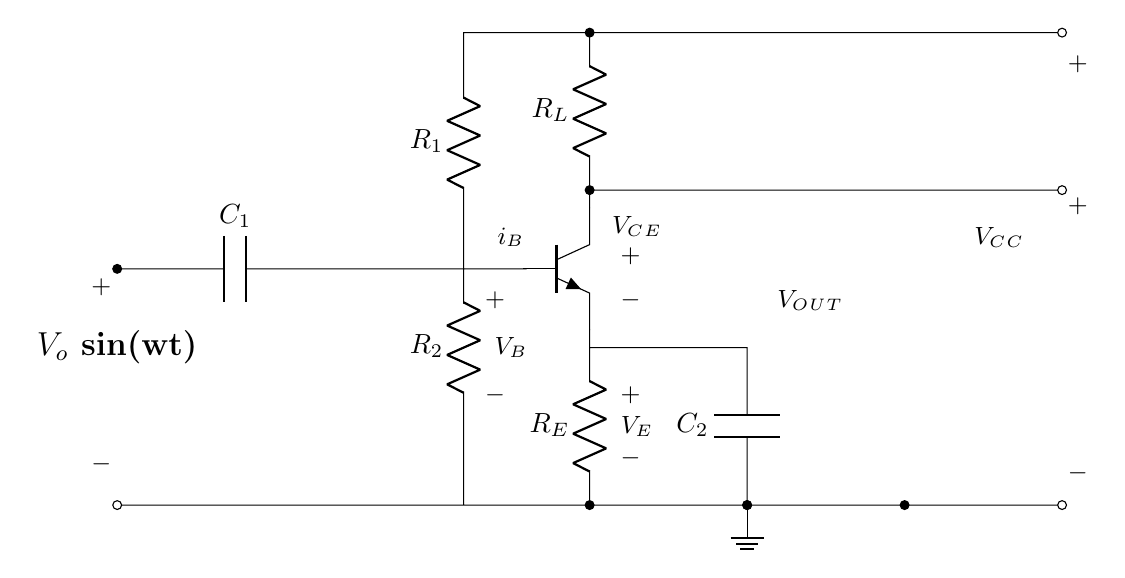
\begin{tikzpicture}[scale=2]
  \draw[color=black]
    (0,0) to [short,o-] (6,0){} 
    (0,1) node[]{\large{\textbf{$V_o$ sin(wt)}}}
    (4,0) node[ground]{} node[circ](3,0){}
    (3.3,1.77) node[]{\small{$V_C$$_E$}}
    (0,1.5) to [C, l=$C_1$, *-] (1.5,1.5)
    to node[short]{}(2.6,1.5)
    (2.2,1.6) to [R, l=$R_1$, -] (2.2,3)
    -| (3,3)
    (1.6,1.5) node[]{\small{\ }}
    (3.3,0.5) node[]{\small{$V_E$}}
    (2.5,1) node[]{\small{$V_B$}}
    (2.5,1.7) node[]{\small{$i_B$}}
    (3,0) to [R,l=$R_E$,*-] (3,1)
    to [Tnpn,n=npn1] (3,2)
    (5.6,1.7) node[]{\small{$V_C$$_C$}}
    (4.4,1.3) node[]{\small{$V_O$$_U$$_T$}}
    (4,0) to [C, l=$C_2$, *-] (4, 1)--(3,1)
    (2.2,0) to [R, l=$R_2$ , - ] (2.2,2)
    (3,2) to [R, l=$R_L$ , - ](3,3)
    to [short,*-o](6,3) 
    (6.1,0.2) node[]{\small{$-$}}
    (6.1,2.8) node[]{\small{$+$}}
    (-0.1,1.38) node[]{\small{$+$}}
    (-0.1,0.26) node[]{\small{$-$}}
    (2.4,1.3) node[]{\small{$+$}}
    (3.26,0.3) node[]{\small{$-$}}
    (3.26,0.7) node[]{\small{$+$}}
    (3.26, 1.3) node[]{\small{$-$}}
    (3.26, 1.58) node[]{\small{$+$}}
    (2.4,0.7) node[]{\small{$-$}}
    (6.1,1.9) node[]{\small{$+$}}
    (3,2)to [short,*-o](6,2)
    (5,0)to [short,*-o](6,0) 
    ;
\end{tikzpicture}
\\
\vspace{1cm}
If you recall JEE Physics, this is a circuit diagram of an npn transistor used as an amplifier. Try your best to match this
circuit. We have used the American voltages convention. It is alright if you can’t get the dimensions to match. What is
important is that you know how to use circuitikz to draw circuits with the components used above, and mark voltages and
currents.
\\
\begin{flushleft}
\Large{\textbf{5 Typesetting exams}}
\end{flushleft}
\\
Congratulations, you’re appointed as a TA for that course you loved last year. The prof, however, is busy with his research,
and wants you to typeset an exam. \textbf{LATEX}, with its exam class can help you do just that!\\

You’ll need to make a separate document, if you want to attempt this task. Your job is to imitate the exam.pdf that we
have provided.\\

\newpage
%%\pagestyle{fancy}\\
\noindent\textbox{Maths\hfill}\textbox{\hfill Assignment\hfill}\textbox{\hfill IIITB \#}
\hline
\vspace{3mm}
\begin{flushleft}
\textbf{Problem 1.}Show that there exists no nontrivial unramified extensions of  $\mathbb{Q}$ .\\
\vspace{3mm}
\textbf{Solution :}If K /$\mathbb{Q}$ is a nontrivial number field,then $\mid disc K \mid > 1$. But then disc K has a prime factor so that some prime ramifies in K.\\
\hspace{19cm}
\framebox[3mm][r]{}\\
\textbf{Problem 2.}Complete the following:\\
\vspace{2mm}
(a) How does one prove a cothereom ? \\
\vspace{0.4cm}
(b) Compute \(\int cosx dx\)\\  
\vspace{0.4cm}
(c) How does one square
$\begin{pmatrix}
a & b \\
c & d 
\end{pmatrix}$?\\
\vspace{0.5cm}
\textbf{Solution:}\\
\vspace{0.5cm}
(a)Use rollaries.\\
\vspace{0.5cm}
(b) We have \\
\hspace{5cm}
\(\int cosx dx = sinx+C\)
 \hspace{9.3cm} (1)\\
 We can check (1):\\
 \hspace{5cm}
 $\frac{d}{dx}{(sinx+C)}$ = $cosx$\\
 \vspace{0.5cm}
 (c) This is routine.\\
 \hspace{19.5cm}\framebox[3mm][r]{}\\
 \vspace{0.1cm}
 \textbf{Problem 3.}Prove that $\sqrt{2}$ is irrational.\\
 \vspace{0.2cm}
 \textit{proof.}Assume that $\sqrt{2}$ =\large{$\dfrac{a}{b}$},where a,b $\in$ $\mathbb{Z}$.Without the loss of generality, we may assume 
$ {\gcd(a,b)}$=\\
 1.Then we have \\
\hspace{6.5cm}  
\vspace{0.2cm}
 $\sqrt{2} = \Large{\dfrac{a}{b}}$\\
\vspace{0.2cm}
\hspace{6.5cm} 
$\sqrt{2}^2 = (\dfrac{a}{b})^2$ \hspace{5cm} (2)\\
\vspace{0.2cm}
\hspace{6.5cm} 
2=\large{$\dfrac{a^2}{b^2}$}\vspace{0.3cm}\\
\hspace{6.5cm}  $a^2$=$2b^2$ \hspace{6cm} (3)\\
\vspace{0.2cm}
 But then from (3),we know that $a^2$ is even so that $a$ is even.But then we must have \\ \vspace{0.2cm}  \hspace{5cm} $ 2a^2 = b^2 $\\
\vspace{0.2cm} 
 so that $b^2$ is even,implying $b$ is even.But then {$gcd(a,b)\ge 2 $},a contradiction.
  \hspace{3cm}
  \framebox[3mm][h]{} \\
\end{flushleft}

%%\fancyfoot[R]{\textbf{1 of 1}}
\vspace{3cm}
\hspace{13cm}\textbf{1 0f 1}
\newpage
\noindent\textbox{CSE 30151 Spring 2016\hfill}\textbox{\hfill Homework 2}
\hline
\usetikzlibrary{automata, positioning,arrows}

(\,b)\,
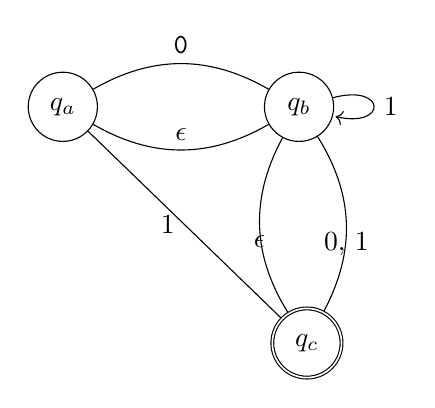
\begin{tikzpicture}
\node[state] (q1) {{$q_a$}};
\node[state, right of=q1,xshift=2cm] (q2) {$q_b$};
\node[state, accepting] at (3.1, -3)(q3) {$q_c$} ;
\draw 
(q1) edge[bend left,above] node{\tt 0}(q2)
(q2) edge[loop right] node{1}(q2)
(q2) edge[bend left, above] node{$\epsilon$} (q1)
(q3) edge[bend left, below] node{$\epsilon$} (q2)
(q3) edge[bend right, below] node{0, 1} (q2)
(q3) edge[below,  left=0.3] node{1} (q1);

\end{tikzpicture}
\section*{4. Solving puzzle\#1}In class, we did three puzzles, the first of which is equivalent to
finite automata. In general, a puzzle of this type has a frame like this (but possibly
with more/fewer squares and different colors):

\vspace{0.5cm}

\centering
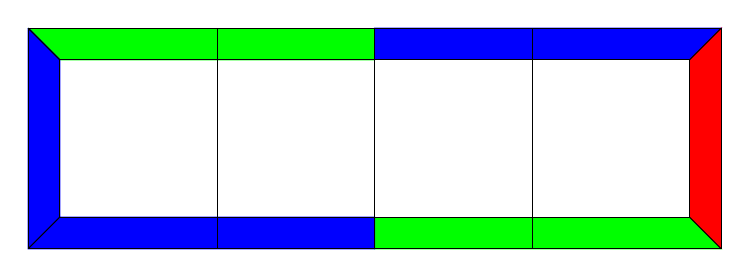
\begin{tikzpicture}

\filldraw[green](-0.4,2.4)--(0,2)--(4,2)--(4,2.4);
\filldraw[green](4,0)--(4,-0.4)--(8.4,-0.4)--(8,0);
\filldraw[blue](4,2)--(4,2.4)--(8.4,2.4)--(8,2);
\filldraw[blue](-0.4,2.4)--(0,2)--(0,0)--(4,0)--(4,-0.4)--(-0.4,-0.4)--(-0.4,2.4);
\filldraw[red](8,0)--(8,2)--(8.4,2.4)--(8.4,-0.4);
\draw (0,0) -- (2,0) -- (2,2) -- (0,2) -- (0,0);
\draw (2,2) -- (4,2) -- (4,0) -- (2,0);
\draw (4,2) -- (6,2) -- (6,0) -- (4,0);
\draw (6,2) -- (8,2) -- (8,0) --(6,0);
\draw (0,0) -- (-0.4,-0.4);
\draw (0,2) -- (-0.4,2.4);
\draw (-0.4,2.4) -- (-0.4,-0.4);
\draw (2,2) -- (2,2.4);
\draw (4,2) -- (4,2.4);
\draw (6,2) -- (6,2.4);
\draw (8,2) -- (8.4,2.4);
\draw(-0.4,2.4) -- (8.4,2.4);
\draw (2,0) -- (2,-0.4);
\draw (4,0) -- (4,-0.4);
\draw (6,0) --( 6,-0.4); 
\draw (8,0) -- (8.4,-0.4);
\draw (-0.4,-0.4) -- (8.4 ,-0.4);
\draw (8.4,-0.4) --(8.4,2.4);
\end{tikzpicture}

\vspace{0.5cm}

And a finite set of tiles like this (but possibly with more/fewer tiles and difent
colors)

\vspace{0.5cm}

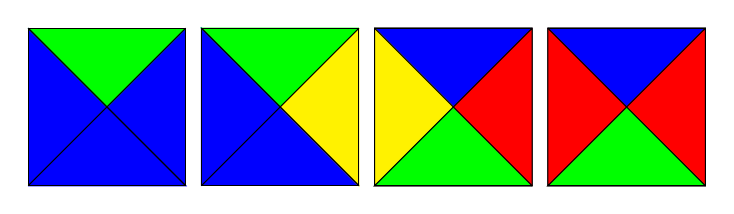
\begin{tikzpicture}

\draw (0,0) -- (2,0) -- (2,2) -- (0,2) -- (0,0);

\filldraw[blue] (0,0) -- (2,0) -- (0,2) ;
\filldraw[blue] (0,0) -- (2,0) -- (2,2) ;
\filldraw[green] (0,2) -- (1,1) -- (2,2);
\draw (0,0) -- (2,2);
\draw (2,0) -- (0,2);
\draw (0,0) -- (2,0) -- (2,2) -- (0,2) -- (0,0);

\draw (2.2,0) -- (2.2,2) --(4.2 ,2) -- (4.2,0)--(2.2,0)  ;
\filldraw[blue] (2.2,0) -- (2.2,2) --(4.2,0) ;
\filldraw[yellow](3.2,1)--(4.2,0)--(4.2,2);
\filldraw[green](3.2,1)--(2.2,2)--(4.2,2);
\draw(2.2,0)--(2.2,2)--(4.2,2)--(4.2,0)--(2.2,0);
\draw (4.2,0)-- (2.2,2);
\draw(2.2,0)--(4.2,2);

\draw (4.4,0)-- (4.4,2) -- (6.4,2) -- (6.4,0)--(4.4,0)--(6.4,2) ;
\draw (6.4,0)-- (4.4,2);
\filldraw[blue] (4.4,2) -- (5.4,1) --(6.4,2) ;
\filldraw[yellow](4.4,0)--(5.4,1)--(4.4,2);
\filldraw[green](4.4,0)--(5.4,1)--(6.4,0);
\filldraw[red](6.4,2)--(5.4,1)--(6.4,0);
\draw (4.4,0)-- (4.4,2) -- (6.4,2) -- (6.4,0)--(4.4,0)--(6.4,2) ;
\draw (6.4,0)-- (4.4,2);



\draw (6.6,0)-- (6.6,2) -- (8.6,2)-- (8.6,0)--(6.6,0)--(8.6,2) ;
\draw (8.6,0) --((6.6,2);
\filldraw[blue] (6.6,2) -- (7.6,1) --(8.6,2) ;
\filldraw[red](8.6,0)--(7.6,1)--(8.6,2);
\filldraw[green](6.6,0)--(7.6,1)--(8.6,0);
\filldraw[red](6.6,2)--(7.6,1)--(6.6,0);

\draw (6.6,0)-- (6.6,2) -- (8.6,2)-- (8.6,0)--(6.6,0)--(8.6,2) ;
\draw (8.6,0) --((6.6,2);
\end{tikzpicture}

\vspace{0.5cm}

The tiles must be arranged so that adjacent areas have matching colors. There is an
unlimited number of copies of each tile.
\vspace{0.1cm}\flushleft
(a) Show how every puzzle of this type can be converted into a finite automaton \textit{M}and a string w such that \textit{M}accepts \textit{w} if and only if the puzzle has a solution.
\flushleft
(b) Apply your construction to the above instance.
\vspace{0.1cm}\flushleft
(c) Briefly describe how this gives an \textit{O(n)} algorithm for solving puzzles of this
type.
\end{document}